\subsection{Plan du campus}
\begin{minipage}{0.7\textwidth}
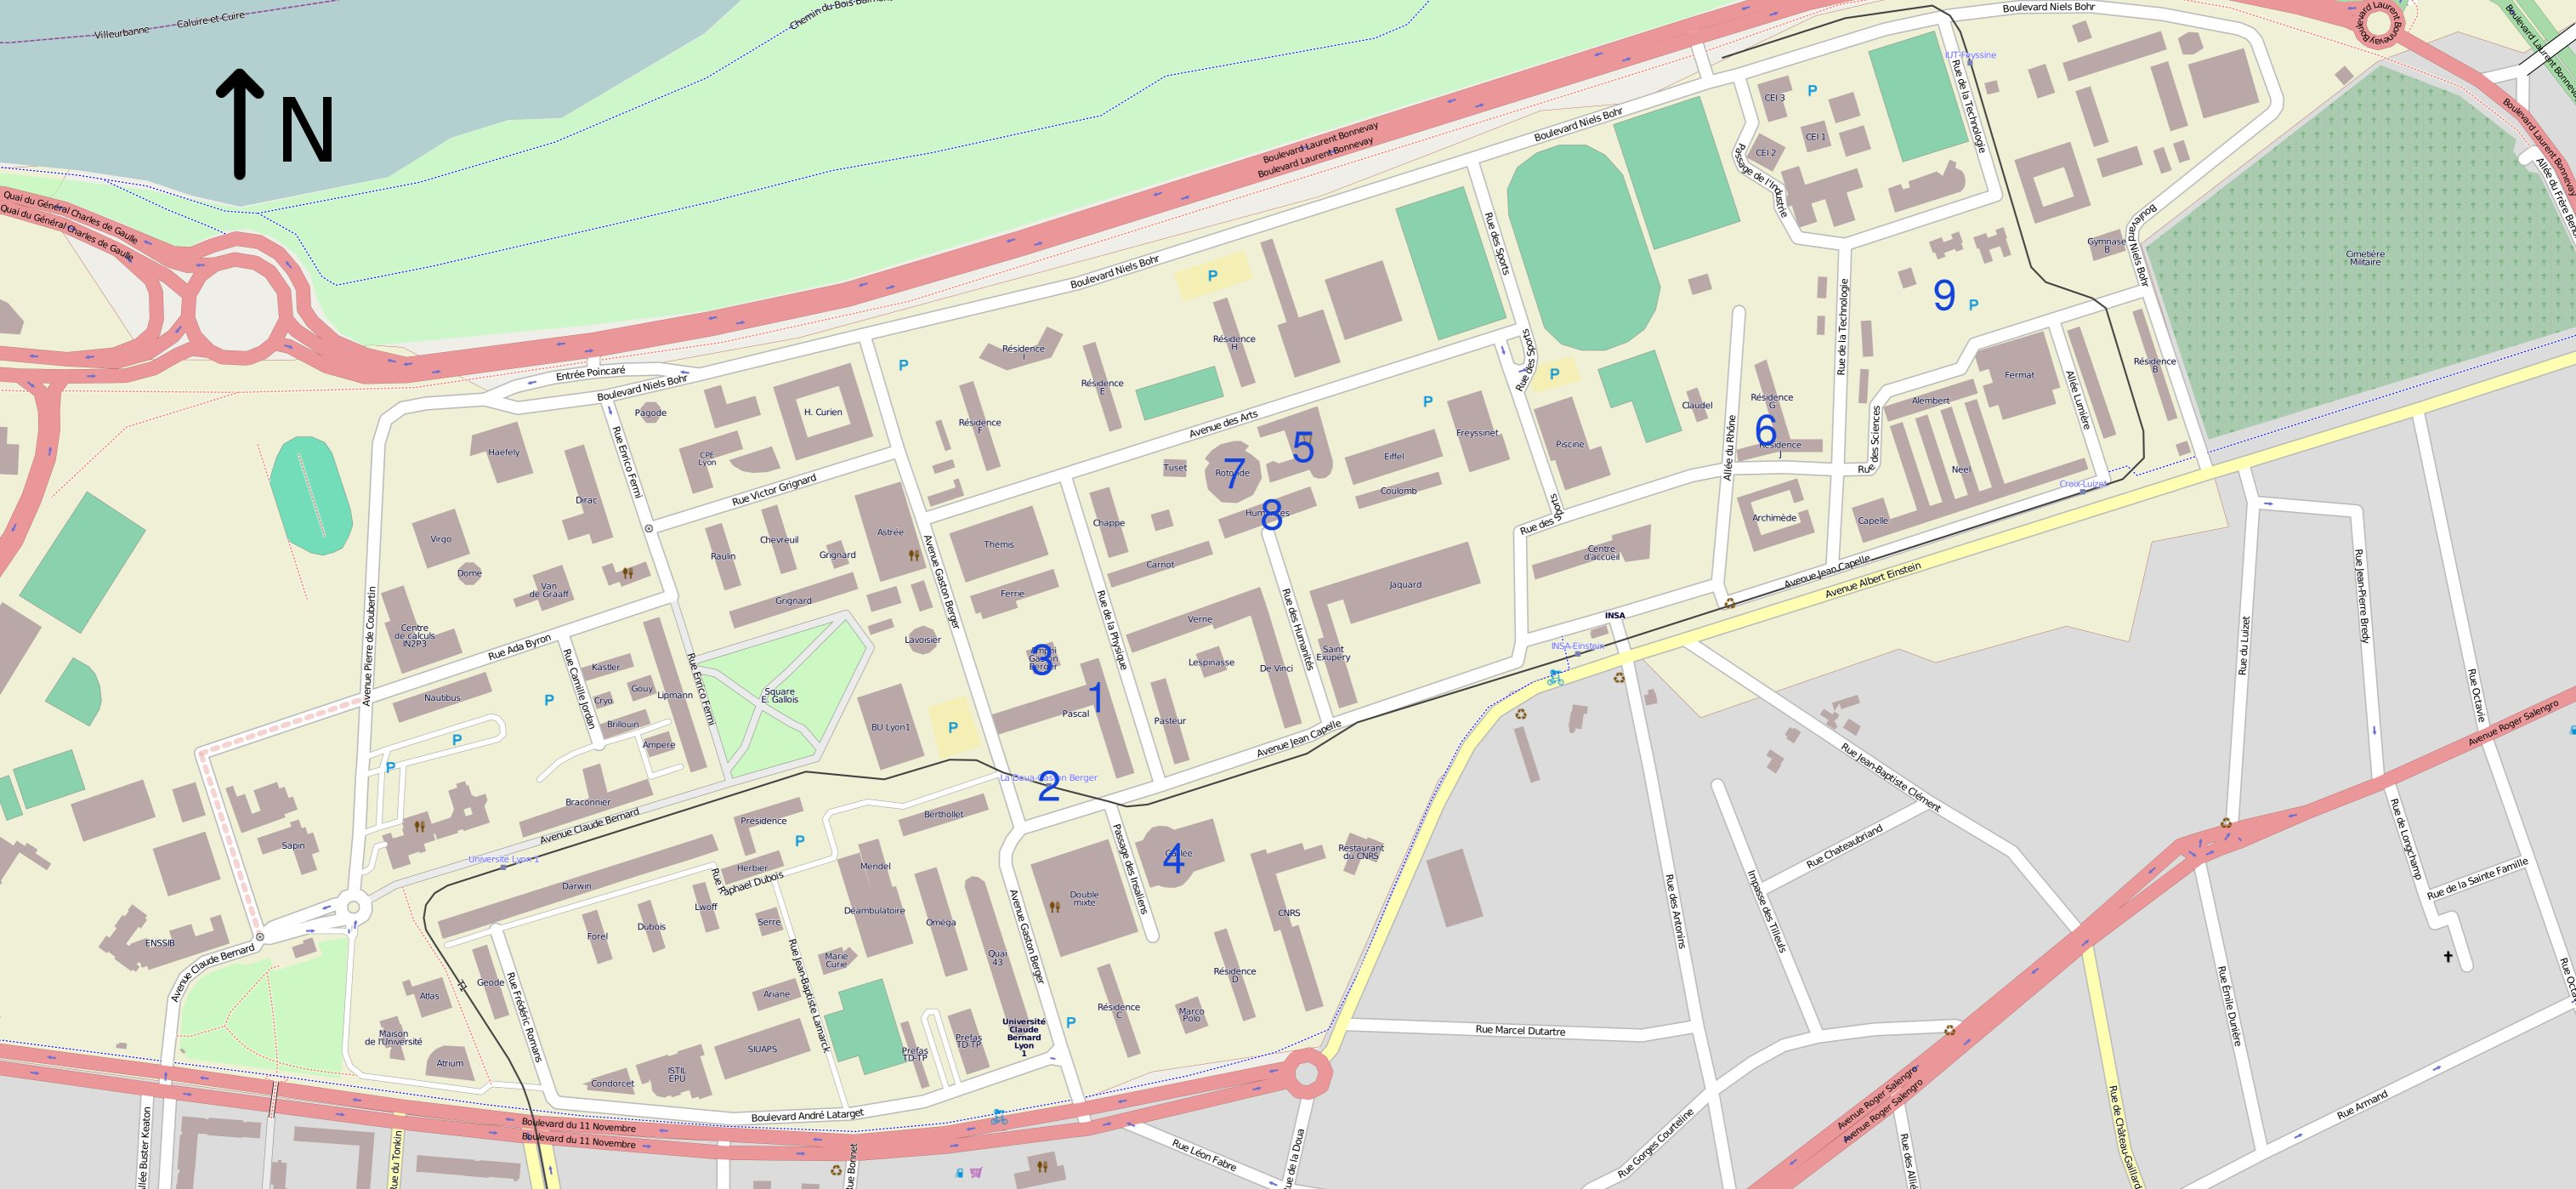
\includegraphics[width=24cm, angle=90]{images/planDoua.jpg}
\end{minipage}
\begin{minipage}{0.3\textwidth}
\textbf{Légende}
    \begin{enumerate}
	\item Département
	\item Amphi
	\item Arrêt de tram
	\item Restaurants
	\item MdE, K-Fêt
	\item Direction des résidences
	\item Rotonde
	\item Bâtiment des Humanités
	\item Bâtiment Pierre de Fermat
    \end{enumerate}
   \vspace{2cm} 
    Il est possible de zoomer sur l'image pour avoir le nom des résidences et
    des bâtiments de manière plus lisible.
\end{minipage}
\newpage

\subsection{Plan TCL}
\hspace{-2cm}
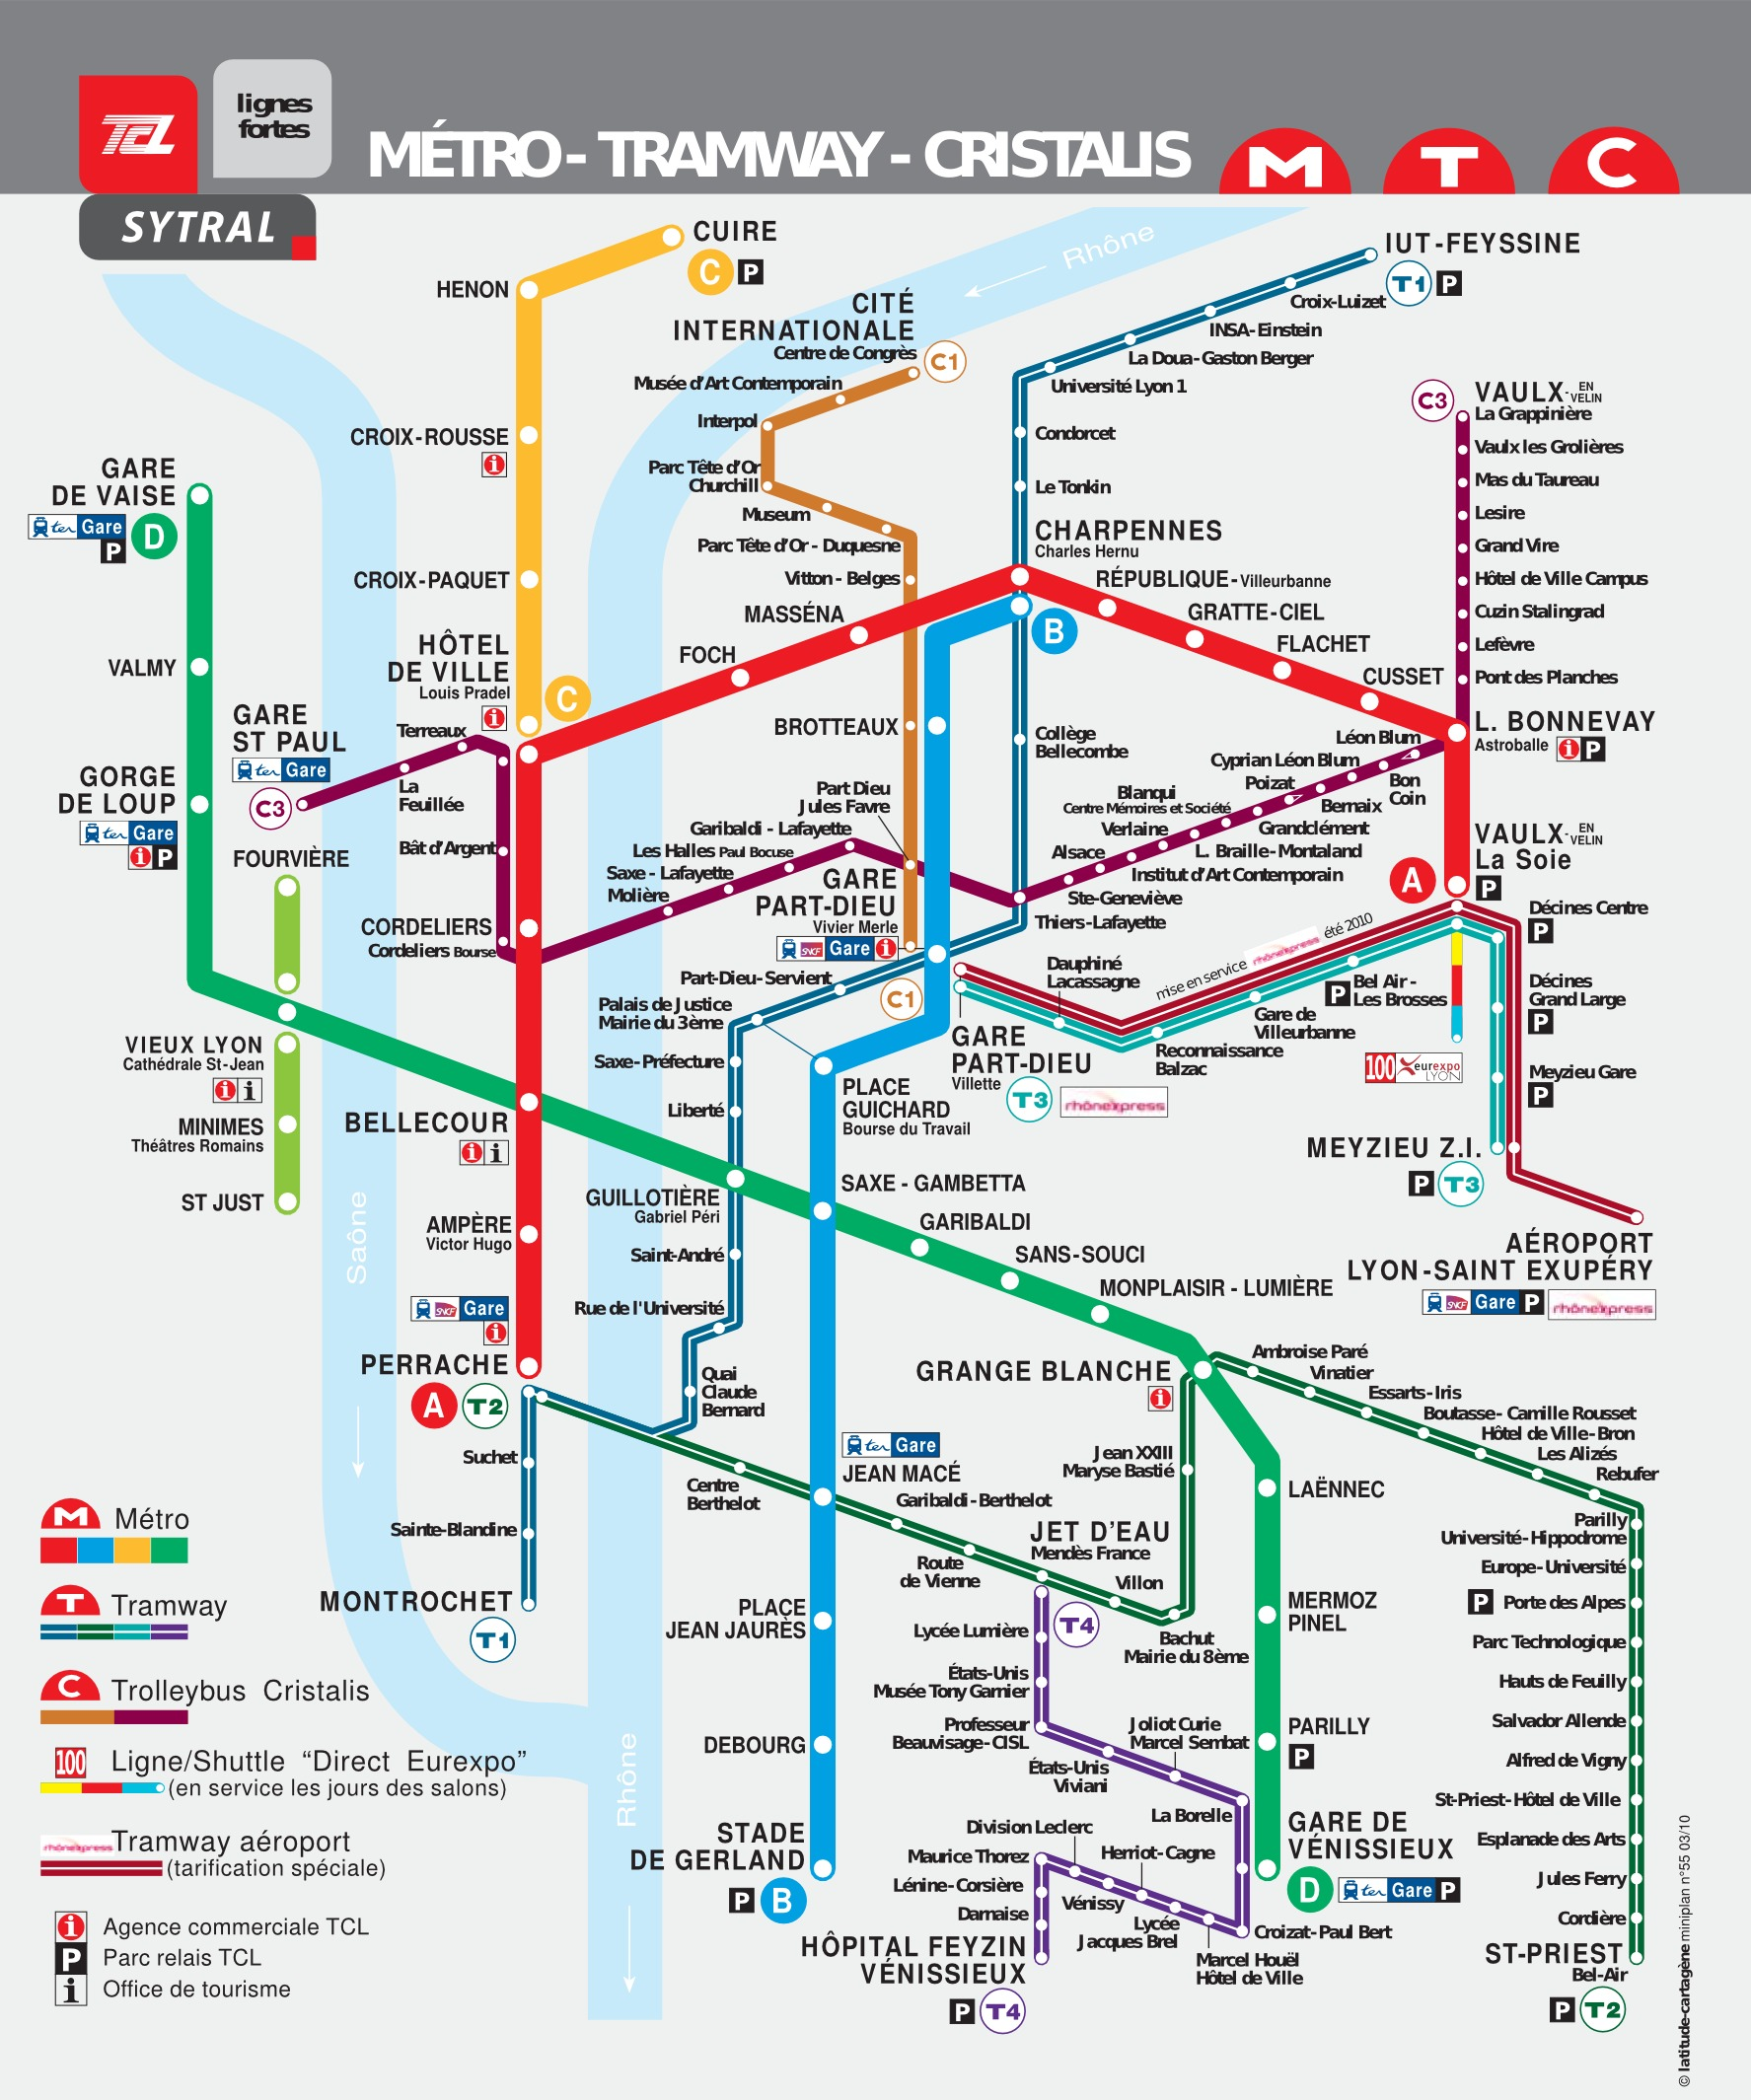
\includegraphics[width=19cm]{images/planTCLFullRes.jpg}

